%%------------------------------------------------------
% 
%% UNIVERSIDADE FEDERAL DE SANTA CATARINA - UFSC
%
%% Prof.: Wyllian B. da Silva
%%
%% Template: estilo IEEEtran [paper com duas colunas]
%% Adaptado de: https://ieeeauthorcenter.ieee.org/create-your-ieee-article/use-authoring-tools-and-ieee-article-templates/ieee-article-templates/templates-for-transactions/
%               https://ctan.org/tex-archive/macros/latex/contrib/IEEEtran?lang=en

%% Instruções: http://mirrors.ctan.org/macros/latex/contrib/IEEEtran/IEEEtran_HOWTO.pdf
%%
%% Recomendações:
%% Utilize o Edito Kile (SO Linux)
%% Certifique-se de que a codificação de caracteres utilizada é a UTF-8





\documentclass[journal]{IEEEtran}


%%------------------------------------------------------
%% Packages
%%------------------------------------------------------
\usepackage[T1]{fontenc}           %% Codificação de caracteres
\usepackage[utf8]{inputenc}        %% Codificação de caracteres (conversão automática dos acentos)
\usepackage[dvips]{graphicx}       %% para a macro includegraphics 
\usepackage[english,brazil]{babel} %% PT_BR e EN (o último define a prioridade no arquivo)
\usepackage{pgf}                   %% macro para criar gráficos
\usepackage{epsfig}                %% or use the epsfig package if you prefer to use the old commands
\usepackage{graphics}              %% use the graphics package for simple commands
\usepackage{graphicx}              %% or use the graphicx package for more complicated commands
\usepackage{epstopdf}              %% enable EPS (convert to PDF)
\usepackage{float}                 %% float environment
\usepackage{eqparbox}              %% to define a group of boxes 
\usepackage{hyphenat}              %% prevent hyphenation
\usepackage{hyperref}              %% enalbe one-click link

% \usepackage{showframe} %% just for the example

% \usepackage[sort,compress]{cite} %% disable if natbib package is activated
\usepackage[numbers,sort&compress,square]{natbib} %% e.g., [2-5]



%%------------------------------------------------------
%% Definitions
%%------------------------------------------------------

\hyphenation{op-tical net-works semi-conduc-tor}

%% Can use something like this to put references on a page
%% by themselves when using endfloat and the captionsoff option.
\ifCLASSOPTIONcaptionsoff
  \newpage
\fi


%%----------------- Definindo as variáveis com números
\makeatletter
%
\newcommand{\prenome}{\afterassignment\prenome@aux\count0=}
\newcommand{\prenome@aux}{\csname prenome\the\count0\endcsname}
%
\newcommand{\nomedomeio}{\afterassignment\nomedomeio@aux\count0=}
\newcommand{\nomedomeio@aux}{\csname nomedomeio\the\count0\endcsname}
%
\newcommand{\sobrenome}{\afterassignment\sobrenome@aux\count0=}
\newcommand{\sobrenome@aux}{\csname sobrenome\the\count0\endcsname}
\makeatother
%%%%%

%%----------------- Configurações de hyperlinks
%% Não decorado, sem destaque
\hypersetup{
  colorlinks=false,
  pdfborder={0 0 0},
}




%%------------------------------------------------------
%% Configurações
%%------------------------------------------------------

%%----------------- Título
\title                                                {Relatório de Programação I}

\newcommand{\emailautor}                              {vinifelssner@gmail.com}

\newcommand{\siglaRevista}                            {UFSC}

\newcommand{\Revista}                                 {Universidade Federal de Santa Catarina (UFSC)}



%%----------------- Autor Principal (a acenturação deverá ser indireta)
\newcommand{\prenomePrincipal}                        {Vinicius}
\newcommand{\nomedomeioPrincipal}                     {dos Anjos}
\newcommand{\sobrenomePrincipal}                      {Felssner}


%%----------------- Demais Autores
%% Segundo autor (a acenturação deverá ser indireta)
\expandafter\newcommand\csname prenome2\endcsname     {Dione}
\expandafter\newcommand\csname nomedomeio2\endcsname  { }
\expandafter\newcommand\csname sobrenome2\endcsname   {Bampi}






%%------------------------------------------------------
%% Autor(es)


%%----------------- Apenas um autor
\author{\IEEEauthorblockN{\prenomePrincipal~\nomedomeioPrincipal~\sobrenomePrincipal\IEEEauthorrefmark{1}}
\prenome2~\nomedomeio2~\sobrenome2\IEEEauthorrefmark{2}

\IEEEauthorblockA{\IEEEauthorrefmark{1}Universidade Federal de Santa Catarina (UFSC)}% <-this % stops an unwanted space
%%
\thanks{\Revista. Correspond\^encia ao autor: \prenomePrincipal~\nomedomeioPrincipal~\sobrenomePrincipal~(email: \emailautor).}}



% %%----------------- Vários Autores
% \author{\IEEEauthorblockN{\prenomePrincipal~\nomedomeioPrincipal~\sobrenomePrincipal\IEEEauthorrefmark{1}, 
% \prenome2~\nomedomeio2~\sobrenome2\IEEEauthorrefmark{2}, 
% \prenome3~\nomedomeio3~\sobrenome3\IEEEauthorrefmark{3}, 
% \prenome4~\nomedomeio4~\sobrenome4\IEEEauthorrefmark{3}, and 
% \prenome5~\nomedomeio5~\sobrenome5\IEEEauthorrefmark{4},~\IEEEmembership{Fellow,~IEEE}}
% 
% \IEEEauthorblockA{\IEEEauthorrefmark{1}Universidade Federal de Santa Catarina (UFSC)}
% 
% \IEEEauthorblockA{\IEEEauthorrefmark{2}School of Electrical and Computer Engineering, Georgia Institute of Technology, Atlanta, GA 30332 USA}
% 
% \IEEEauthorblockA{\IEEEauthorrefmark{3}Starfleet Academy, San Francisco, CA 96678 USA}
% 
% \IEEEauthorblockA{\IEEEauthorrefmark{4}Tyrell Inc., 123 Replicant Street, Los Angeles, CA 90210 USA}% <-this % stops an unwanted space
% %%
% \thanks{\Revista~(\siglaRevista). Correspond\^encia ao autor: \prenomePrincipal~\nomedomeioPrincipal~\sobrenomePrincipal~(email: \emailautor).}}



%%------------------------------------------------------
%% Cabeçalho
\markboth{\MakeUppercase{\Revista}}%% acentuação indireta
%% Apenas um autor:
{\sobrenomePrincipal: \MakeUppercase{\Revista}}
%% Mais de um autor:
% {\sobrenomePrincipal: \MakeLowercase{\textit{et al.}}: \Revista}


%%------------------------------------------------------
%% Abstract
\IEEEtitleabstractindextext{

  {\selectlanguage{brazil}
    \begin{abstract}
    O projeto se baseia em fazer uma jogo escrito na linguagem c, utilizando o sistema operacional Linux com a distro Mint,o jogo deve rodar no Konsole, para esse projeto foram usadas duas bibliotecas padrões do c, a stdio.h e stdlib.h. O jogo é do estilo estratégia, possuí três fases e cutscenes para contar a história. A gameplay usa as teclas W, A, S, D e H, cada uma possuindo uma função diferente.
    \end{abstract}
    %%----------------- Keywords
    \renewcommand\IEEEkeywordsname{Palavras-chave} %% Palavras-chave ao invés de 'Index Terms'
    \begin{IEEEkeywords}
    Jogo, Projeto, Linguagem C, Konsole, Stdio.h, Stdlib.h, Três fases, Estratégia, Cutscenes, Gameplay, Mint.
    \end{IEEEkeywords}
  }

  {\selectlanguage{english}
    \begin{abstract}
    The project is based in make a game write in c language, using the Linux with distro Mint as a operational system, the game must work in Konsole or Terminal, for this project were used two standart headers from c language, the stdio.h and stdlib.h. It is a strategy game , there are three levels, and cutscenes to tell the story, The gameplay use the keys W, A, S, D and H each having a different function.
    \end{abstract}
    %%----------------- Keywords
    \begin{IEEEkeywords}
    Game, Project, C language, Konsole, Stdio.h, Stdlib, , Three Levels, Strategy, Cutscenes, Gameplay, Mint.
    \end{IEEEkeywords}
  }
}








\begin{document}



%%------------------------------------------------------
%% Inserção de informações
\maketitle
\IEEEdisplaynontitleabstractindextext
\IEEEpeerreviewmaketitle


%%------------------------------------------------------
%% Section
\section{Introdução}
\IEEEPARstart{E}{ste} relatório tem o objetivo de explicar todos os passos de como foi planejado e executado o projeto do  jogo, o qual se trata de um trabalho de Programação I.
O nome escolhido para o jogo foi Strange World, o intuito inicial era fazer um jogo de tiro, com a câmera com visão de cima, semelhante ao jogo Grand Theft Auto, de 1997, desenvolvido pela DMA Design, outra característica importante definida foi que o jogo teria múltiplas decisões durante a sua história e se passaria em um mundo pós-apocalíptico. Detalhes sobre o desenvolvimento do jogo serão dados a seguir. 
\begin{figure}[!htbp]
\centering
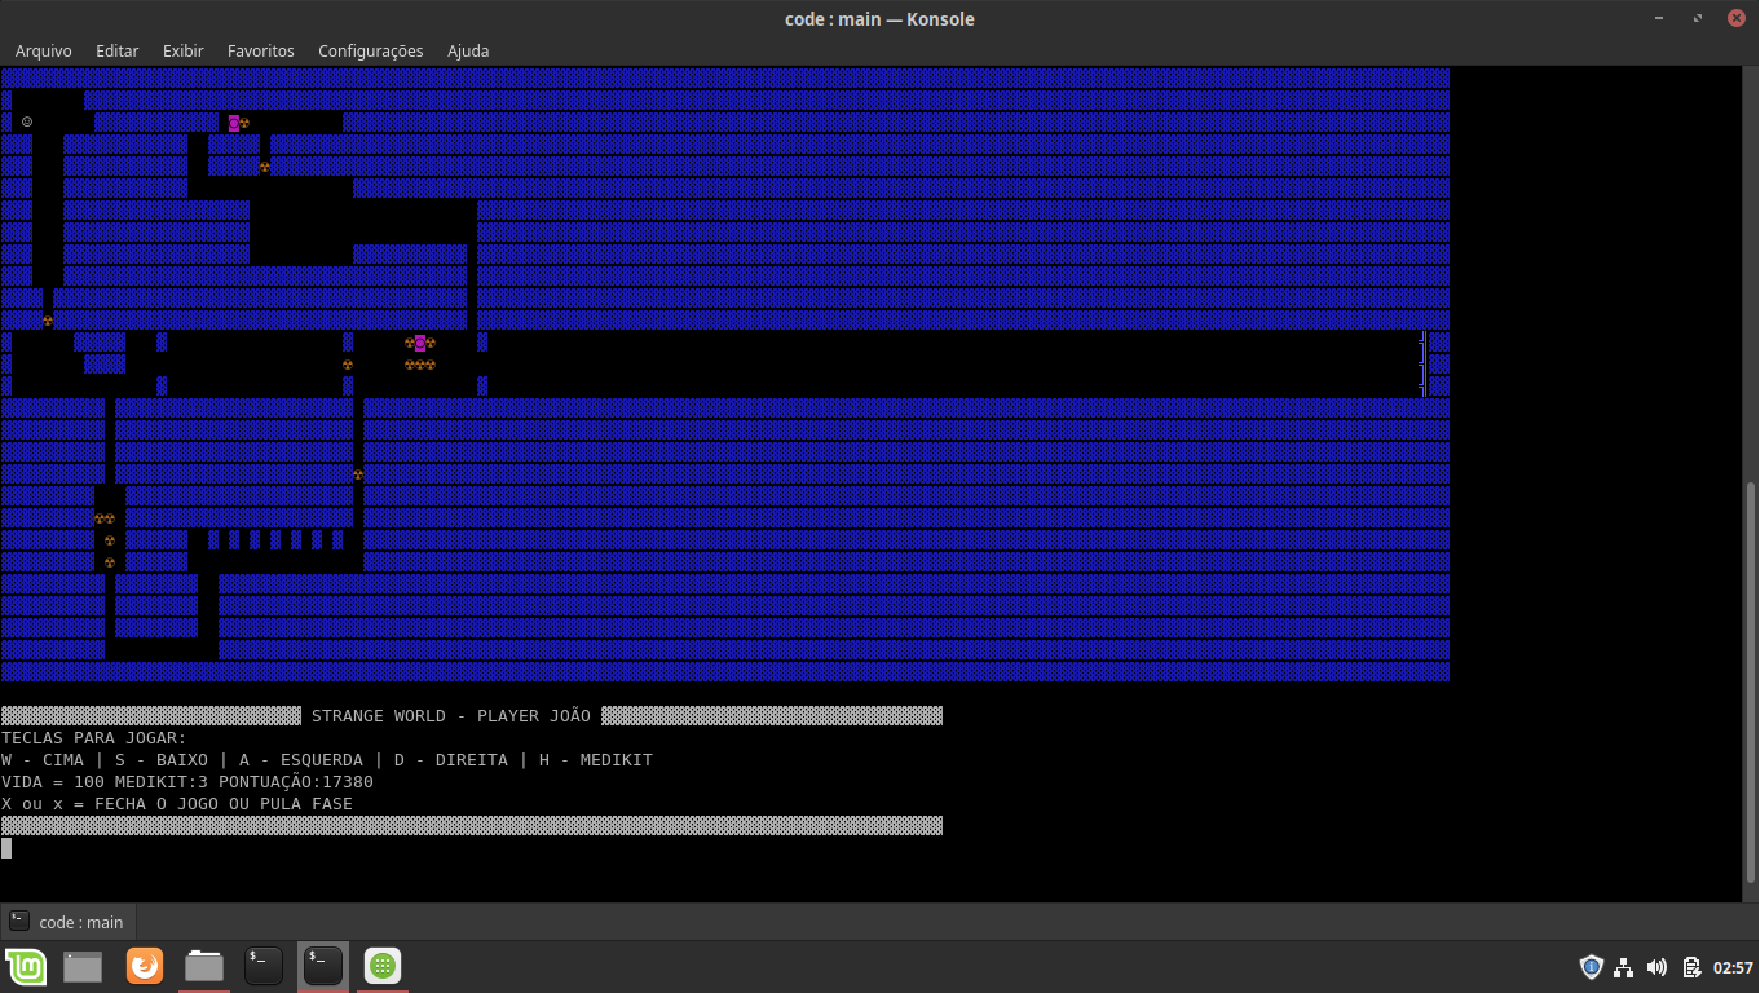
\includegraphics[width=.50\columnwidth]{figs/png2pdf.pdf}
\caption{Cenário do Jogo.}
\label{fig:fig_exemple}
\end{figure}

O jogo se chama Strange World a Figura~\ref{fig:fig_exemple} é uma captura de tela do cenário 3, onde há obstaculos e hameplay interativa com o cenáario, utilizando as teclas referidas é possível navegar pelomenu e assim iniciar o jogo, após o início o jogador será recebido por algumas cutscenes as quais contam o enredo e posteriormente é inicida a parte jogável, as teclas de ações são W, A, S, D e H, cada uma possuindo sua respectiva função e assim o jogo se desenrola entre diferentes fases e cutscenes. 




%%------------------------------------------------------
%% Section
\section{Metodologia}
A criação do projeto foi iniciada após alguns dias de diálogo e pesquisas, onde várias ideias foram expostas e discutidas, para assim decidir o que seria feito e o que era melhor não levar adiante.
As decisões sempre foram tomadas buscando obter um equilibro entre complexidade e viabilidade, o que acabou excluindo muitas ideias por serem assumidas como muito complexas de serem executadas ou, por outro lado, por serem muito simples.
Depois de já definido como seria o jogo, se deu inicio à execução, o método escolhido foi por partes, começando pelo menu e seguindo, respectivamente, por: Um cenário simplificado inicial, os cenários do jogo, a parte escrita do jogo, a implementação de movimento e a organização do código.


%%------------------------------------------------------
%% Section
\section{Resultados ou Resultados Experimentais ou Resultados Esperados}
O inicio da execução se deu pelo menu, onde foi relativamente rápido de se executar, o material encontrado na internet foi abundante e de fácil compreensão, foi utilizado na criação estruturas de if e printf.
Na execução do cenário simplificado e dos cenários do jogo, aconteceram vários problemas, foi encontrado pouco material a respeito na internet, e os poucos encontrados ou eram muito complexos ou não eram funcionais para o nosso propósito, após alguns dias de tentativas, os cenários foram deixados de lado e inciamos a execução da história do jogo.
A história do jogo foi executada sem problemas, embora foi necessário um longo periodo para ser terminada. Para cria-la foram utilizados, vetores, printfs e programas de edição de imagens e conversão para ASCII, principalmente usados na criação das cutscenes.
Em seguida, iniciamos simultaneamente a execução dos cenários e da implementação da movimentação, após um periodo de tentativas e falhas, conseguimos criar um cenário simplificado e implementar o movimento de um caractere no interior desse cenário. O proximo passo foi criar os cenários definitivos do jogo, seguindo do conhecimento aplicado no cenário simplificado e do estudo de um código de um jogo de labirinto encontrado no site www.vivaolinux.com.br, conseguimos criar um cenário inicial, que veio a ser a fase 1 do jogo, para a criação foram uitilizados matrizes, estruturas de define, for, if, printf, e outras de menor relevancia para o código.
A criação do cenário e a implementação da movimentação nele foram feitos praticamente simultaneamente, a partir disso, com menu, cenário 1 e movimentação prontos, se deu inicio à organização do código, definindo quais partes seriam funções separadas e como seria a main.
Por fim, seguindo o modelo do cenário 1, foram criados os cenários 2 e 3, utilizando as mesmas estrururas da linguagem C usadas no cenário 1.
No intervalo entre a criação do cenário 1 e dos outros dois, tentamos implementar um sistema de tiros, onde o personagem João atiraria para matar os inimigos pelo mapa, que era o intuito incial do jogo, infelizmente não conseguimos e optamos por implementar um sistema de estratégia, mudando o perfil do jogo para um estilo mais RPG.
É importante também mencionar que a implementação da história do jogo, seguiu desde o seu incio após o termino do menu, até o fim do código, compartilhando o  tempo de trabalho com as outras etapas que foram sendo executadas paralelamente.
No final tentamos implementar alguns sons, como música de fundo e beeps, mas não conseguimos.
Depois de todas as partes do código prontas e organizadas, terminamos o tempo de trabalho com o código e passamos para a criação do vídeo e deste relatório.


%%------------------------------------------------------
%% Section
\section{Conclusão ou Conclusões}
Ao fim deste trabalho de programação, pudemos concluir e entender uma infinidade de aplicações da programação de computadores, mais específicamente da linguagem C, mas além disso, perceber que ainda há muito mais para se aprender.
Encontramos situações que julgamos significantenente complexas na execução deste trabalho, e embora não consguimos resolver cem por cento delas, com o conhecimento adquirido em sala de aula e o material pesquisado fora dela, nós conseguimos resolver a maior parte das situações e executarmos o projeto do jogo até o final.
Concluímos que neste trabalho adquirimos uma muito maior familiaridade com a linguagem C.






\end{document}
